\label{sec:foundations_of_query_processing}

There is considerable work in database systems, from architectures and techniques for transaction and query processing to data models, languages, and user interfaces. This section focuses primarily on query processing and gives a comprehensive overview of what techniques currently exist. It focuses mainly on fundamental query processing mechanisms of relational databases that use declarative languages, such as \gls{sql}.

\subsection{Architecture of a Query Processor}

Figure \ref{fig:query_processor} shows the traditional architecture for query processing and the different steps this process involves. When the query processor receives a \gls{sql} statement as input, the query is translated into an internal representation to be further optimized to reduce the overall execution runtime. Finally, the selected execution plan is submitted to the \gls{dbms} execution engine to obtain the desired result. We present a brief description of each component below.

\begin{figure}[ht]
\centering
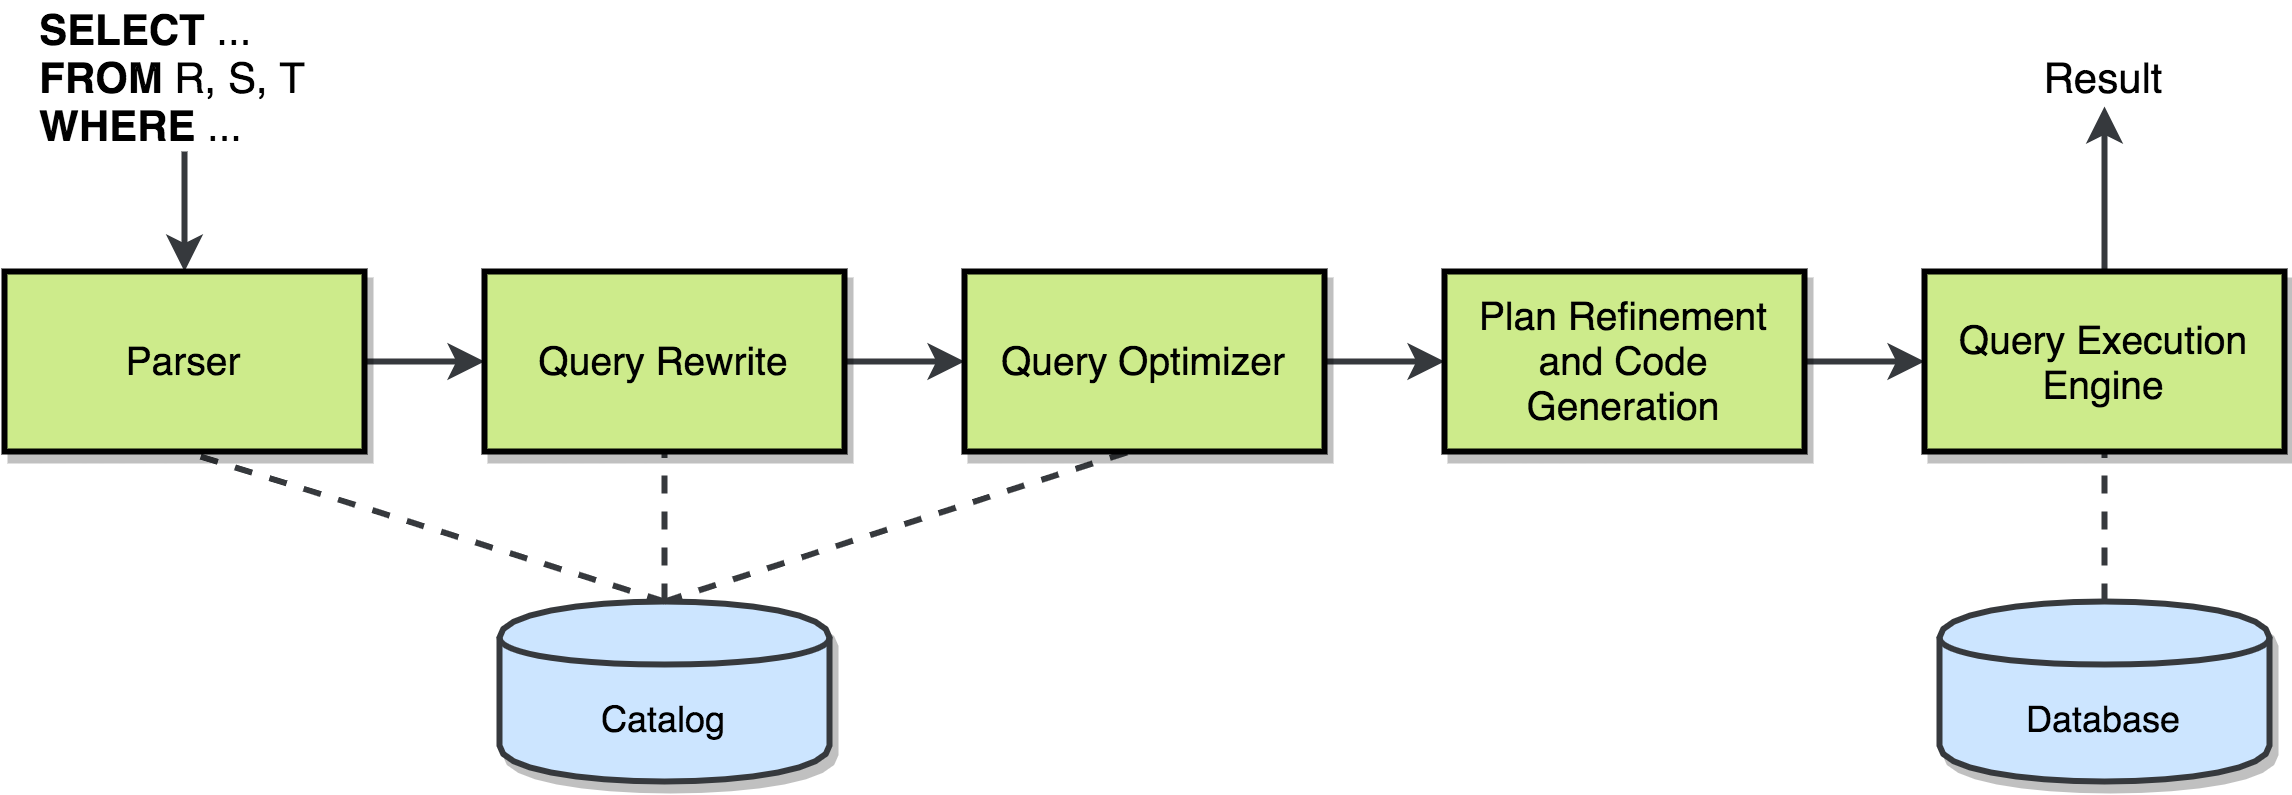
\includegraphics[width=0.95\textwidth]{img/state_of_the_art/architecture_of_a_query_processor.png}
\caption{Query processing steps \citep{Kossmann2000}}
\label{fig:query_processor}
\end{figure}

\subsubsection{Parser}

As the \gls{sql} statement itself provides an abstraction to lower-level details, it needs to be parsed and translated into an internal representation to be later optimized. This is the primary function of the parser.

\subsubsection{Query Rewrite}

In this stage, multiple transformation rules that do not depend on the system's physical state are applied. Such rules are good choices regardless of the size of the tables, the existence of index structures, locations of copies of tables, and computational power. This process includes eliminating redundant predicates, simplifying expressions, and \textit{unnesting} subqueries. % In a distributed system, the selection of table partitions must also be taken into account.

\subsubsection{Query Optimizer}

The query optimizer applies transformations that depend on the physical state of the system. For example, it determines the indices to use when executing the query, the methods (e.g., hashing or sorting) to use when executing the operations involved (e.g., joins and group-bys), and the order in which they should be executed. %Additionally, in a distributed system, the optimizer determines where each operation should be carried out. 
These decisions are made following a cost model and enumerating several alternative execution plans that return the same result.

\subsubsection{Plan}

A plan specifies how a particular query should be executed. Generally, query plans resemble traditional tree structures. Each node represents a query operator (e.g., join, group-by, sort, scan), and the edge between nodes represents the parent-child relationship between them. %In distributed systems, these can be annotated, indicating, for example, where an operator should be executed.

\begin{figure}[ht]
\centering
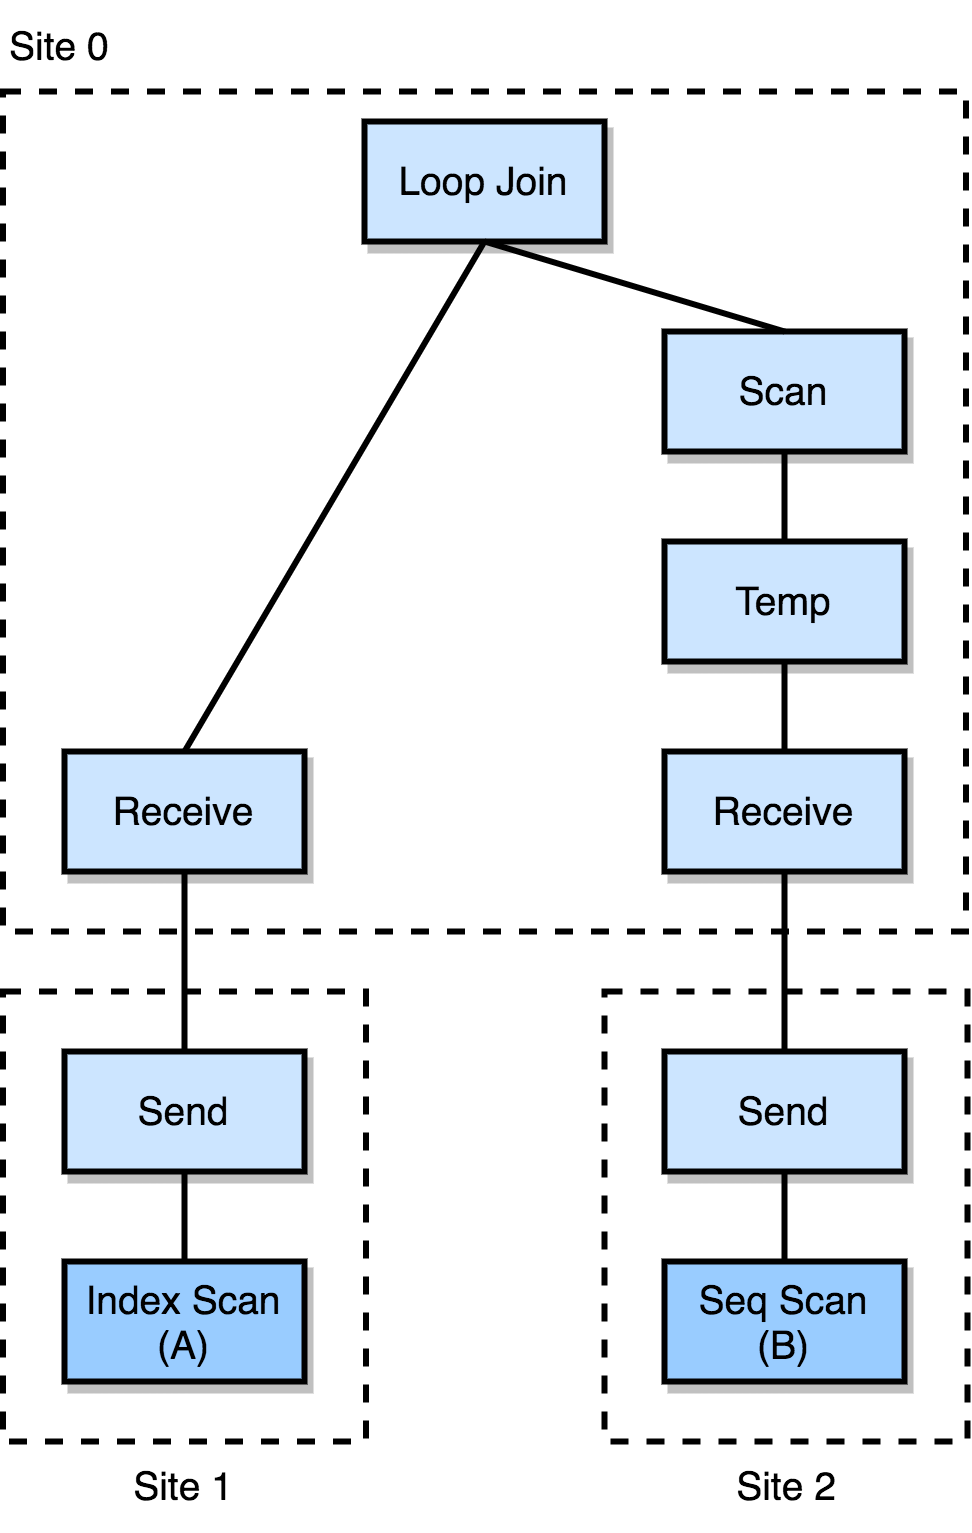
\includegraphics[width=0.4\textwidth]{img/state_of_the_art/execution_plan.png}
\caption{Example of a query execution plan \citep{Kossmann2000}}
\label{fig:execution_plan}
\end{figure}

Figure \ref{fig:execution_plan} shows an example execution plan for a query that involves two different Tables: $A$ and $B$. It specifies that \textit{Table A} is scanned at \textit{Site 1} using an index, and $B$ is scanned at \textit{Site 2}. They are then shipped to \textit{Site 0} using \textit{send} and \textit{receive} operators, and $B$ is materialized and reread at \textit{Site 0}. Both tables are then joined using a nested-loop join operator.

\subsubsection{Plan Refinement and Code Generation}

In the plan refinement and code generation stage, the plan produced by the optimizer in the previous step is transformed so that it can be further interpreted and executed by the query execution engine.

\subsubsection{Query Execution Engine}

This component ensures that generic implementations for every operator (e.g., send, scan or nested-loop join) exist. Current query execution engines are based on an iterator model \citep{Graefe1993b}, where operators are implemented as iterators that share the same interface. This allows combining two different iterators (following the consumer-producer relationship of a plan), meaning that any plan can be executed. Another advantage of the iterator model is that it supports the pipelining of results from one operator into another to improve query execution performance.

\subsubsection{Catalog}

As mentioned earlier, the optimization effectiveness depends on statistics regarding the state of the database. The catalog stores all the information needed for optimization. It maintains the database schema, partitioning schema, and physical information about the database. In traditional relational database systems, the catalog information is stored in tables. %In a distributed environment, different approaches can be considered when it comes to catalog storage. The most obvious one is to store the catalog at one central site. However, it may make sense to replicate the catalog at several sites to reduce communication costs. Nevertheless, as the catalog's size grows and is frequently updated, one strategy taken into account is to store various partitions of catalog data where it is most needed.

\bigbreak

\noindent It is important to note that, even though the architecture represented in Figure \ref{fig:query_processor} is the most widely used today, other alternatives have emerged over time. For example, many commercial database systems use architectures such as Volcano \citep{Graefe1993} and Cascades \citep{Graefe1995}, where query rewriting and optimization steps proceed as one.

Query processors may also differ in various aspects, such as the optimization granularity. For instance, there have been proposals to optimize multiple queries at a time \citep{Sellis1988}. This approach can be efficient if the queries are similar, even if the search space significantly increases.

\subsection{Basic Optimization Approach and Techniques}
\label{sec:basic_optimization_approach}

This section addresses the basic approach and strategies for optimizing queries. It first explains how a dynamic programming algorithm enumerates alternative query execution plans and then defines how different cost models can be used to estimate a particular plan's execution cost.

\subsubsection{Plan Enumeration with Dynamic Programming} 
\label{sec:dynamic_programming}

In this type of approach, the execution plan is created at compile-time and only later executed by the \gls{dbms} engine. The conventional strategy to optimize this type of queries goes back to the dynamic programming algorithm used in System R \citep{Selinger1979} and is currently implemented in most commercial systems.

\begin{figure}[ht]
\begin{algorithm}[H]
\SetAlgoLined
\DontPrintSemicolon
\KwIn{$QT$: query tree with $n$ relations}
\KwOut{$output$: best QEP (Query Execution Plan)}
\Begin{
 \For{each relation $R_i \in QT$}{
    \For{each access path $AP_{ij}$ to $R_i$}{
        compute cost($AP_{ij}$)\;
    }
  best $AP_i \longleftarrow AP_{ij}$ with minimum cost\;
  \For{each order ($R_{i1}, R_{i2},...,R_{in}$) with $i = 1,...,n!$}{
    build QEP (...((best $AP_{ij} \bowtie R_{i2}) \bowtie R_{i3}) \bowtie ... \bowtie R_{in}$)\;
    compute cost (QEP)\;
  }
  $output \longleftarrow$ QEP with minimum cost\;
 }
}
\caption{Plan Enumeration with Dynamic Programming}
\end{algorithm}
\caption{Simplified version of the dynamic programming algorithm \citep{Ozsu2011}}
\label{fig:dynamic_programming}
\end{figure}

The simplified version of the algorithm is shown in Figure \ref{fig:dynamic_programming}. It involves two loops that operate in a bottom-up fashion, building more complex plans through simpler ones. In the first step, the optimizer selects the best access method for each table referenced in the query. To do so, it exploits the predicates and access paths available for each table and estimates the cost for each alternative plan. For instance, if a hypothetical Table $A$ is replicated in sites $S_1$ and $S_2$, the algorithm would enumerate $scan (A, S_1)$ and $scan (A, S_2)$ as two possible alternatives to use in the final plan.

If the query involves more than a single table, the optimizer will explore all possible join sorting permutations ($n!$ possibilities for $n$ relations). Permutations are produced by the dynamic construction of a tree with alternative strategies. It is relevant to mention that the algorithm does not consider all possible permutations since some are not of interest. For example, permutations involving Cartesian products and the commutative equivalent strategies with the highest cost are not considered. With these two heuristics, the number of strategies examined has an upper bound of $2^n$ rather than $n!$. Inefficient plans are discarded (i.e., pruned) as soon as possible. A plan can be discarded when there is an alternative at a lower cost. For example, $A \bowtie B$ and $B \bowtie A$ would be considered two possible alternatives, but only one of them would be considered in the optimal plan. This step reduces the complexity of query optimization as it prevents more complex plans from being obtained from simpler and inefficient ones.

\subsubsection{Cost Model and Cardinality Estimation}

An optimizer's cost model predicts the cost of a given execution plan and relies on functions to predict the cost of operators, statistics and base data, and formulas to evaluate the size of intermediate results. Using cardinality estimates as its primary input, estimating the cost of a particular query execution plan typically includes estimating the cost of all operators involved and summing them up.

Cardinality estimates are usually computed based on simplifying assumptions such as uniformity and independence. The principle of uniformity assumes that all values, except for the most common ones, have the same number of tuples. On the other hand, the principle of independence assumes that predicates on attributes are independent. For joins, certain cardinality estimators follow the principle of inclusion, where the domains of the join keys overlap such that the keys from the smaller domain have matches in the larger domain.

\subsection{Dynamic Optimization Approach and Techniques}
\label{sec:dynamic_optimization_approach}

Even though the traditional approach outlined in the previous section is widely accepted, there has been a concern over the years that cost estimates lead to too many errors since many data sources do not provide reliable statistics about the system's state. Since certain assumptions made at compile-time rarely hold throughout query processing, the accuracy of the information the optimizer considers changes over time. In addition, specific parameter values may not be known until runtime. For this reason, questions about the timing of the optimization were raised, and adaptive query processing techniques were developed, allowing execution plans to be altered at execution time.

\paragraph{Dynamic Query Evaluation Plan}

\citep{Cole1994} introduced the idea of generating several alternative plans or sub-plans at compile-time, save them in the database and choose the plan that best fits the state of the system right before its execution. The approach is primarily static given that dynamic execution plans are initially produced using a dynamic programming algorithm as the one described earlier in Section \ref{sec:dynamic_programming}. However, certain optimization decisions may occur at runtime. For instance, it is possible to use choose-plan operators when two different plans are incomparable. Two or more equivalent plans are incomparable at compile time when important runtime information (e.g., parameter bindings) is missing to estimate cost.

\paragraph{Decomposition}

\citep{Ozcan1997} developed a strategy for processing queries where the general procedure consists of two steps. First, in query decomposition, the query is rewritten into a group of sub-queries, each targeted at a single data source, based on information acquired on the fly. Second, the query scheduler explores the potential parallelism and execution dependencies between the different sub-queries to restrain the search space and optimal query execution schedule. This minimizes the overall response time and, consequently, reduces the total query processing cost.

\paragraph{Continuously Adaptive Query Processing}

Eddies \citep{Avnur2000} is a query optimization system that continuously reorders operators in a query plan as it runs by merging the optimization and execution stages. This allows each tuple to have a flexible ordering of the query operators. It is possible for query plans to be reordered using two different principles: (1) synchronization barriers where inputs from different sources are coordinated and (2) moments of symmetry where pipelined joins are easily reordered.